\documentclass[11pt,a4paper]{article}
\usepackage[T1]{fontenc}
\usepackage[utf8]{inputenc}
\usepackage{lmodern}
\usepackage{amsmath,amssymb,amsthm,mathtools,mathrsfs}
\usepackage{graphicx,float,xcolor,multicol}
\usepackage[shortlabels]{enumitem}
\usepackage[margin=27mm]{geometry}
\usepackage{microtype,needspace,placeins}
\usepackage{tikz,tikz-cd}
\usetikzlibrary{arrows.meta,calc,positioning,patterns,decorations.pathreplacing}
\usepackage[colorlinks=true,linkcolor=teal,urlcolor=teal,citecolor=teal]{hyperref}
\setlength{\parindent}{0pt}
\setlength{\parskip}{.6em}
\setcounter{secnumdepth}{0}
\allowdisplaybreaks
\raggedbottom
\providecommand{\cross}{\times}
\DeclareUnicodeCharacter{2020}{\ensuremath{\dagger}}
\DeclareMathOperator{\supp}{supp}
\DeclareMathOperator*{\esssup}{ess\,sup}
\providecommand{\chapter}{\section}
\newenvironment{tool}[2]{\subsection*{Tool #1 --- #2}}{}
\newcommand{\ToolRef}[1]{Tool #1}
\newcommand{\FigureTag}[2]{\textit{Figure #1}}
\newcommand{\Result}[1]{\subsection*{#1}}
\newcommand{\Application}[1]{\subsubsection*{Application\if\relax\detokenize{#1}\relax\else\space--- #1\fi}}
\newcommand{\ProofHeading}{\par\textit{Proof.}\space}
\newcommand{\ProofOf}[1]{\par\textit{Proof of #1.}\space}
\newcommand{\RemarkHeading}{\par\textbf{Remark.}\space}
\newcommand{\NoteHeading}{\par\textbf{Note.}\space}
\newcommand{\ExerciseHeading}{\par\textbf{Exercise.}\space}

% Rendering support only; mathematical text is in each independent post.
\usepackage{booktabs,array,longtable}
\definecolor{HandoutBlue}{HTML}{2F6690}
\definecolor{HandoutNavy}{HTML}{17365D}
\newtheorem{theorem}{Theorem}
\newtheorem{lemma}[theorem]{Lemma}
\newtheorem{proposition}[theorem]{Proposition}
\newtheorem{corollary}[theorem]{Corollary}
\newtheorem{conjecture}[theorem]{Conjecture}
\newtheorem{definition}{Definition}
\newtheorem{example}{Example}
\newtheorem{namedtoolcounter}{Tool}
\newenvironment{namedtool}[1]{\begin{namedtoolcounter}[#1]}{\end{namedtoolcounter}}
\newtheorem*{claim}{Claim}
\newtheorem*{remark}{Remark}
\newtheorem*{exercise}{Exercise}
\newtheorem*{question}{Question}
\newtheorem*{observation}{Observation}
\newcommand{\SourceChapter}[2]{\section*{#2}}
\newcommand{\Lecture}[2]{\section*{Lecture #1: #2}}
\newcommand{\unclear}[1]{\textit{[unclear: #1]}}
\newcommand{\sourcegap}{\textit{[unfinished in the source]}}
\DeclareMathOperator{\dist}{dist}
\DeclareMathOperator{\id}{id}
\DeclareMathOperator{\Hol}{Hol}
\DeclareMathOperator{\Per}{Per}
\DeclareMathOperator{\Fix}{Fix}
\DeclareMathOperator{\diam}{diam}
\DeclareMathOperator{\Var}{Var}
\DeclareMathOperator{\Leb}{Leb}
\DeclareMathOperator{\Hom}{Hom}
\DeclareMathOperator{\End}{End}
\DeclareMathOperator{\Ann}{Ann}
\DeclareMathOperator{\Spec}{Spec}
\DeclareMathOperator{\Max}{Max}
\DeclareMathOperator{\Ob}{Ob}
\DeclareMathOperator{\Tor}{Tor}
\DeclareMathOperator{\Ass}{Ass}
\DeclareMathOperator{\Mor}{Mor}
\DeclareMathOperator{\Fun}{Fun}
\DeclareMathOperator{\Nat}{Nat}
\DeclareMathOperator{\Cone}{Cone}
\DeclareMathOperator{\MCG}{MCG}
\DeclareMathOperator{\Aut}{Aut}
\DeclareMathOperator{\Deck}{Deck}
\DeclareMathOperator{\SL}{SL}
\DeclareMathOperator{\PSL}{PSL}
\DeclareMathOperator{\Area}{Area}
\DeclareMathOperator{\im}{im}
\DeclareMathOperator{\PSh}{PSh}
\newcommand{\CRing}{\mathsf{CRings}}
\newcommand{\AMod}{A\text{-}\mathsf{Mod}}
\newcommand{\Ab}{\mathsf{Ab}}
\newcommand{\Z}{\mathbb Z}
\newcommand{\Q}{\mathbb Q}
\newcommand{\R}{\mathbb R}
\newcommand{\C}{\mathbb C}
\newcommand{\N}{\mathbb N}
\newcommand{\kk}{\mathbb k}
\renewcommand{\aa}{\mathfrak a}
\newcommand{\bb}{\mathfrak b}
\newcommand{\pp}{\mathfrak p}
\newcommand{\qq}{\mathfrak q}
\newcommand{\mm}{\mathfrak m}
\newcommand{\nn}{\mathfrak n}
\newcommand{\rad}{\mathrm r}
\newcommand{\cat}[1]{\mathsf{#1}}
\setcounter{secnumdepth}{0}
\allowdisplaybreaks

\graphicspath{{figures/lemma-book/}}
\begin{document}
\section*{Isogonal Conjugates and Pole–Polar Geometry}
% BLOG-CONTENT-BEGIN
\subsection{Isogonal conjugates}
% Source page 2 - right (left is inside cover)
I am back with a tantalizing, appetizing feast of mathematical insight!
Let us begin with the intriguing concept of isogonal conjugates.
\setcounter{theorem}{97}\begin{lemma}[Isogonal conjugates]\label{lemma:lb2-101}
Given a point $P$ inside triangle $ABC$, reflect $AP,BP,CP$ in the angle bisectors of $A,B,C$.
The resulting lines are concurrent. Their point of concurrence is the isogonal conjugate of $P$ in triangle $ABC$.
\end{lemma}
\begin{figure}[H]\centering
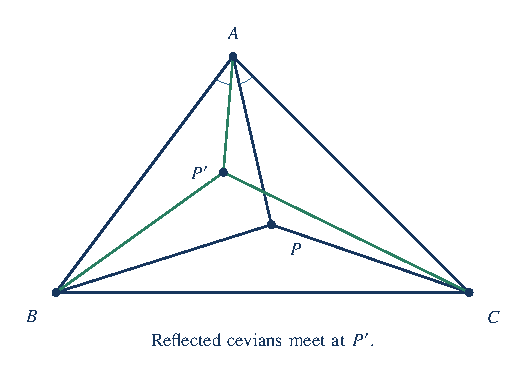
\includegraphics[width=.67\linewidth]{lb2-fig-01.pdf}
\FigureTag{LB2.1}{fig:lb2-01}
\end{figure}
The circumcentre and orthocentre are isogonal conjugates of each other, while the incentre is its own isogonal conjugate.
\paragraph{Application.}

For those who did not read Volume 1---how dare you!---here is the problem.
% Source page 3 - left
\paragraph{IMO (1996).}
In triangle $ABC$, an interior point $P$ satisfies
$\angle APB-\angle C=\angle APC-\angle B$.
Prove that the bisectors of $\angle PBA$ and $\angle PCA$, together with $AP$, concur.
\begin{figure}[H]\centering
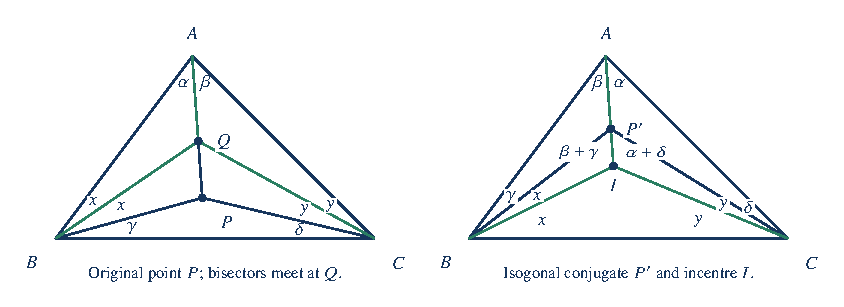
\includegraphics[width=.84\linewidth]{lb2-fig-02.pdf}
\FigureTag{LB2.2}{fig:lb2-02}
\end{figure}
The angle condition on $P$ gives $\alpha+\delta=\beta+\gamma$.
Angle bisectors concur to give the incentre; therefore $AP$ and the bisectors of $\angle ABP$ and $\angle ACP$ are concurrent.
``Game's over.'' The two points shown on $AP$ need not coincide.
% Source page 3 - right
\paragraph{Guess that! Pythagoras Olympiad (1980).}
In triangle $ABC$, a point $D$ satisfies
$\angle DCA=\angle DCB=\angle DBC=10^\circ$ and $\angle DBA=20^\circ$.
Find $\angle CAD$.
\begin{figure}[H]\centering
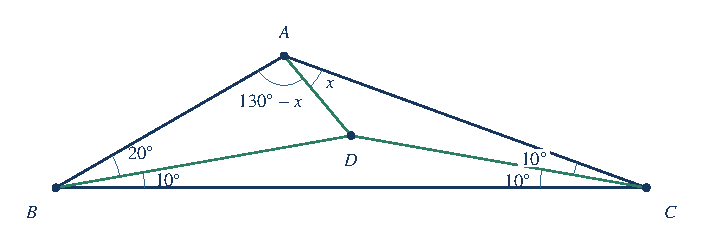
\includegraphics[width=.79\linewidth]{lb2-fig-03.pdf}
\FigureTag{LB2.3}{fig:lb2-03}
\end{figure}
``Sometimes we get lucky!'' Apply trigonometric Ceva:
\[
\frac{\sin x}{\sin(130^\circ-x)}\frac{\sin20^\circ}{\sin10^\circ}
\frac{\sin10^\circ}{\sin10^\circ}=1
\Longrightarrow\frac{\sin x}{\sin(130^\circ-x)}
=\frac{\sin10^\circ}{\sin20^\circ}=\frac1{2\cos10^\circ}.
\]
Quickly guess $x=30^\circ$. To write it formally, note
\[
\frac12\frac1{\cos10^\circ}
=\sin30^\circ\frac1{\sin100^\circ},
\quad\frac{\sin30^\circ}{\sin100^\circ}
=\frac{\sin x}{\sin(130^\circ-x)}
\Longrightarrow x=30^\circ.
\]
It is still not fully general; anyway, it is a novel but nonsense method!

\setcounter{theorem}{98}\begin{lemma}[Concurrent perpendiculars]\label{lemma:lb2-102}
Let $A,B,C$ form a triangle and $P,Q,R$ be three points in the plane.
The lines through $P,Q,R$ perpendicular to $BC,CA,AB$, respectively, are concurrent if and only if
$BP^2-PC^2+CQ^2-QA^2+AR^2-RB^2=0$.
\end{lemma}
% Source page 4 - left


\setcounter{theorem}{102}\begin{lemma}[Trigonometric Ceva]
In triangle $ABC$, the lines $AD,BE,CF$ are concurrent if and only if
$\sin\angle BAD\sin\angle ACF\sin\angle CBE
=\sin\angle DAC\sin\angle BCF\sin\angle ABE$.
\end{lemma}


\subsection{Pole and polar argument}
To master PAPA techniques, begin with the standard definitions.
\begin{figure}[H]\centering
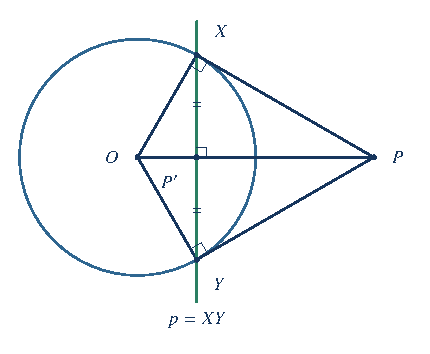
\includegraphics[width=.70\linewidth]{lb2-fig-09.pdf}
\FigureTag{LB2.9}{fig:lb2-09}
\end{figure}
In the drawing, $P$ is the pole of $XY$ and the line $p=XY$ is the polar of $P$.
Here are three magical properties of PAPA. Draw the figures yourself for a better picture!
\setcounter{theorem}{103}\begin{lemma}[La Hire's theorem: PAPA I]\label{lemma:lb2-106}
Let $x,y$ be the polars of $X,Y$, respectively. Then $X$ lies on $y$ if and only if $Y$ lies on $x$.
\end{lemma}
\setcounter{theorem}{104}\begin{lemma}[Intersection of polars: PAPA II]\label{lemma:lb2-107}
Let $x,y,z$ be the polars of $X,Y,Z$. Then $Z=x\cap y$ if and only if $z=XY$.
\end{lemma}
\setcounter{theorem}{105}\begin{lemma}[Complete quadrilateral: PAPA III]\label{lemma:lb2-108}
Let $W,X,Y,Z$ lie on a circle. If $P=XY\cap WZ$, $Q=WX\cap ZY$, and $R=XZ\cap YW$,
then the polar of $P$ is $QR$. Similarly, the polar of $Q$ is $PR$.
\end{lemma}
% Source page 12 - left
I was amazed by Akopyan's presentation of geometry theorems.
His book, \emph{Geometry in Figures}, is probably one of the best on Olympiad geometry.
Let us adopt his style for some PAPA applications!
\Needspace{29\baselineskip}
\paragraph{Problem 1.}
Prove $RS\perp UV$.
\begin{figure}[H]\centering
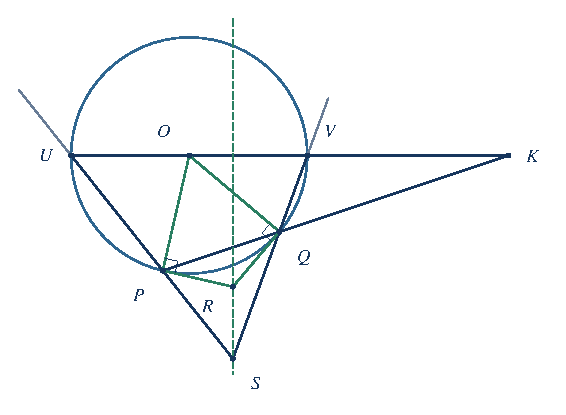
\includegraphics[width=.78\linewidth]{lb2-fig-10.pdf}
\FigureTag{LB2.10}{fig:lb2-10}
\end{figure}
$K$ lies on $r$, so $R$ lies on $k$ by PAPA I, La Hire's theorem.
$S$ lies on $k$ by PAPA III, so $k=RS$ and $RS\perp UV$.
\emph{Quite quickly done.}
Imagine the source: it appeared in the Chinese Mathematical Olympiad!
% Source page 12 - right
\paragraph{Problem 2.}
Prove that $P,E,F$ are collinear.
\begin{figure}[H]\centering
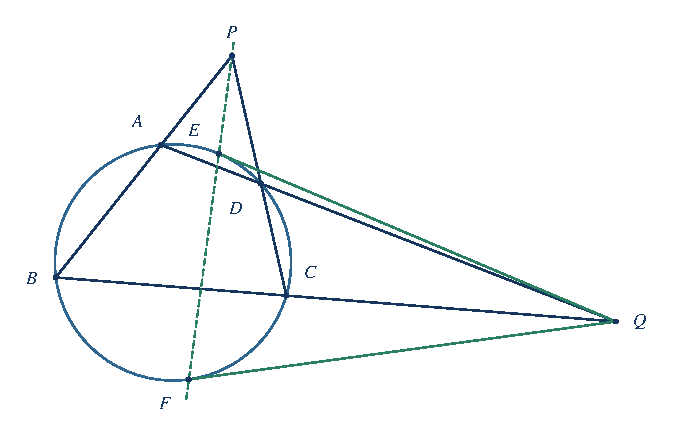
\includegraphics[width=.78\linewidth]{lb2-fig-11.pdf}
\FigureTag{LB2.11}{fig:lb2-11}
\end{figure}
By definition, $q=EF$. By PAPA III, $P$ lies on $q$.
Therefore $P,E,F$ are collinear. \emph{Quite quickly done.}
This also appeared in the Chinese Mathematical Olympiad, in 1997!
\paragraph{Challenge.}
Solve the fourth geometry problem of the IMO Shortlist 2009 using PAPA.
% BLOG-CONTENT-END
\end{document}
